{% -*- mode: LaTeX; TeX-PDF-mode: t; TeX-master: "manual"; -*-
}

\chapter{\ei Clients}
\label{ch:clients}

This chapter describes the different clients available in the \ei
framework. Currently the only mature one is the web-client that we
describe in Section~\ref{ch:clients:web}. The Eclipse and remote shell
clients are under development.

\section{The Web-Client}
\label{ch:clients:web}

\begin{figure}[h]
\hrule\smallskip
\begin{center}
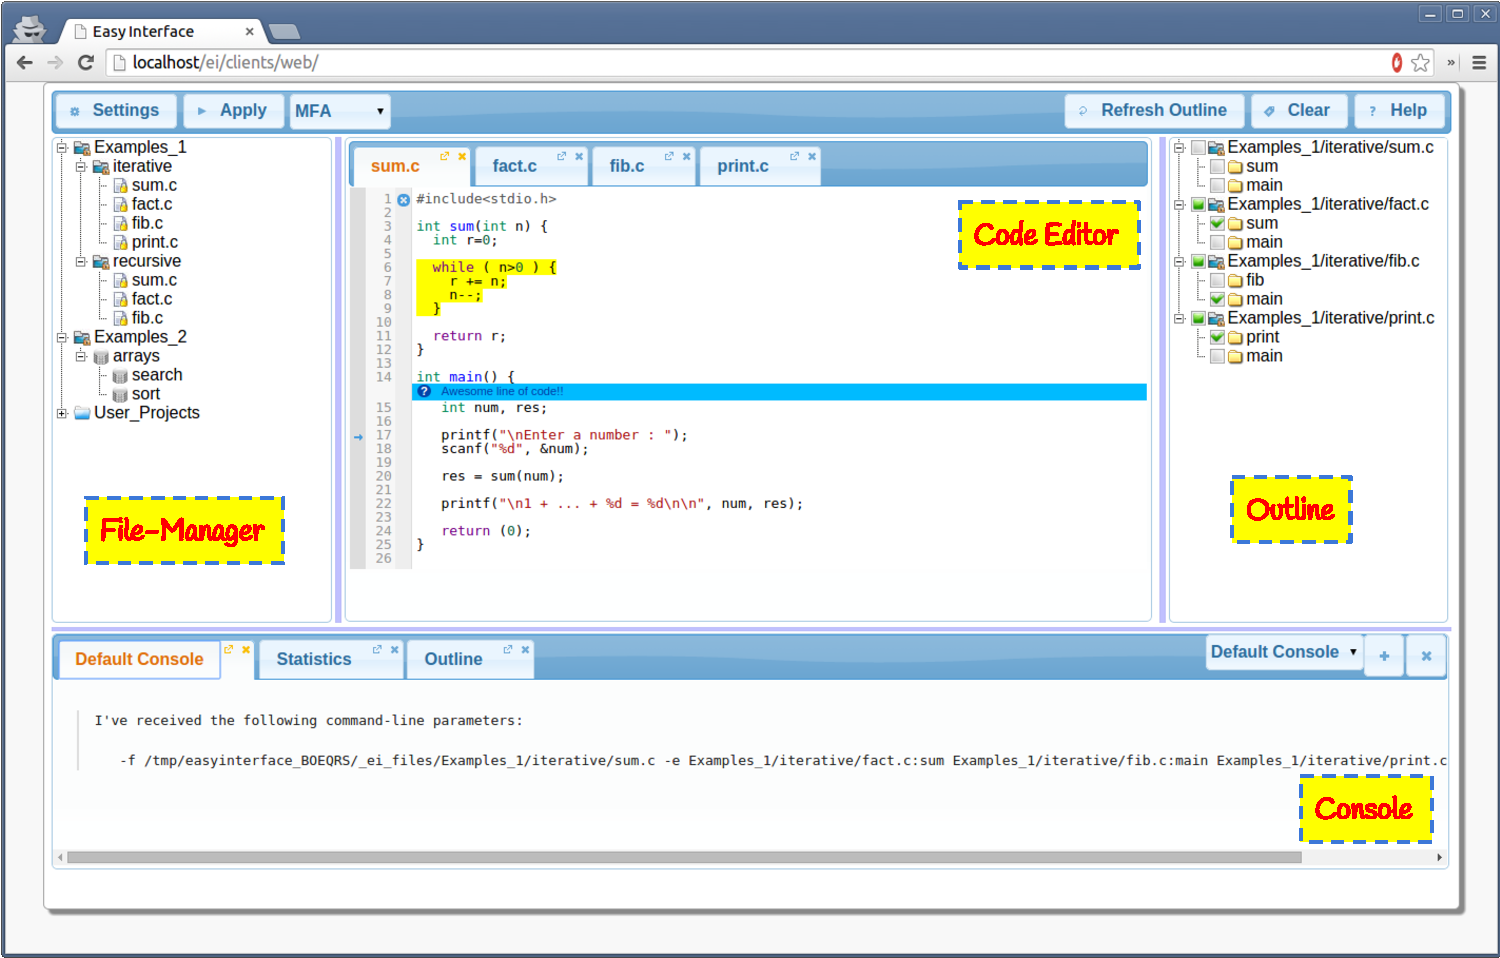
\includegraphics[width=1\textwidth]{fig/webclient.pdf}
\end{center}
\caption{\ei Web Client}
\label{fig:webclient}
\hrule
\end{figure}

The web-client of \ei is a JavaScript program that runs in a web
browser. To access it simply visit
\url{http://localhost/ei/clients/web} and you will get a page similar
to that of Figure~\ref{fig:webclient}.
%
This page has 5 main components: (1) the code area, where users can
edit programs; (2) the file-manager that contains a list of predefined
examples as well as user files; (3) the outline that includes an
outline of one or more files; (4) the console area where the results of
executing an application is printed; (5) the tools bar that includes
several buttons to execute an application, etc.

The web-client can be configured to fit your needs, it has a
configuration file to control (1) which applications to include in the
applications menu; (2) which examples to show in the file-manager; and
(3) how to generate the outline for a set of programs.
%
The web-client first looks for the configuration file
\texttt{clients/web/webclient.cfg}, and if it does not exists it uses
\texttt{clients/web/webclient.default.cfg}.
%
It is recommended not to substantially change
\texttt{webclient.default.cfg}, and instead create your own
\texttt{webclient.cfg}.
%
Next we explain the different components of the configuration file. In
what follows, when we refer the \emph{default server} we mean the one
that is available at the same address as web-client, i.e., if the
web-client was accessed using the URL
``\lst{http://somedomain/.../ei/client/web}'' then the URL of the
default server is ``\lst{http://somedomain/.../ei/server}''.

The configuration file is a text file that includes a single JSON
record with several fields. Let us explain it using the following
complete record:

\bigskip
\begin{lstlisting}
{
  (*title*): (*"Easy Interface"*),
  (*apps*): (*[\{server: "http://domain/.../ei/server, apps: ["myapp", "costa", "mhp"]\}, ... ]*),
  (*examples*): (*[\{server: "http://domain/.../ei/server, examples: ["mhpex","costex"]\}, ... ]*),
  (*outline*):(*"on"*),
  (*outlineserver*): (*"http://domain/.../ei/server"*),
  (*outlineapp*): (*"coutline"*)
}
\end{lstlisting}

\bigskip
\noindent
All fields in the above record are optional, the web-client assigns
default values for those that are not available. 
%
The field \texttt{title} is used to set the window title (see
Figure~\ref{fig:webclient}), where its default value is ``Easy
Interface''. The field \texttt{apps} is used to change the set of
application to be listed in the applications menu, it is explained in
Section~\ref{ch:clients:web:appsmenu}. The field \texttt{examples} is
used to change the set of examples that are shown in the file-manager,
it is explained in Section~\ref{ch:clients:web:filemanager}. The
component called outline at the Figure~\ref{fig:webclient} could be
hide with the field \texttt{outline} when gets ``off'' value. The
fields \texttt{outlineserver} and \texttt{outlineapp} are used to
indicate which application to use for generating the content of the
outline when the \texttt{outline} is active, it is explained in
Section~\ref{ch:clients:web:outline}.

\subsection{The Applications Menu}
\label{ch:clients:web:appsmenu}

The application menu, the combo-box next to the \applybutton button in
Figure~\ref{fig:webclient}, includes a list of applications that can
be executed by the user. This list can be modified by setting the
value of the filed \texttt{apps} in the configuration file. This value
is a list of JSON records of the form

\bigskip
\begin{lstlisting}
  { (*server: SRV, apps: APPSLIST*) }
\end{lstlisting}
 
\bigskip
\noindent  
where \lst{SVR} is a URL to an \ei server and \lst{APPSLIST} is a list
of application identifiers (see \xmlstructref{server}{app}).
%
\lst{APPSLIST} can also be the special value \lst{_all} which refers
to all application of the corresponding server.
%
The default value of this field is a list with a record that refers to
all applications of the default server.

\subsection{The File-Manger}
\label{ch:clients:web:filemanager}

In the file-manager area, of Figure~\ref{fig:webclient}, you can see a
tree-view that represents programs on which the applications can be
applied, etc. The one with the name \texttt{User\_Projects}
corresponds to programs that are created by the user; and the rest are
predefined set of examples. This set of example can be modified by
setting the value of the field \texttt{examples} in the configuration
file.  This value is a list of JSON records of the form

\bigskip
\begin{lstlisting}
  { (*server: SRV, examples: EXLIST*) } 
\end{lstlisting}

\bigskip
\noindent
where \lst{SVR} is a URL to an \ei server and \lst{EXLIST} is a list
of example set identifiers (see
\xmlstructref{server}{exset}). \lst{EXLIST} can also be the special
value \lst{_all} which refers to all example sets of the corresponding
server. The default value of this field is a list with a record that
refers to all example sets of the default server.

\subsection{The Outline}
\label{ch:clients:web:outline}

The outline area of Figure~\ref{fig:webclient} includes a tree-view
that represents information on some programs, e.g., methods, classes,
etc. The actual values in this tree and its structure depend very much
on the intended use of \ei, and thus, it is completely configurable.
%
The idea is that the user will select some of the entries in this
tree, and then they will be passed to the application that we apply
(see Section~\ref{ch:quickguide:outline}
and~\xmlstructref{server}{cmdlineapp}).

The actual content of the outline is not generated by the web-client,
but rather by an external application that is installed on some \ei
server that we refer to as the \emph{outline application}. It like any
other application but typically non-visible.  The exact work-flow for
generating an outline is as follows:
%
\begin{enumerate}

\item the user clicks on the \refreshoutline button to generate an
  outline for the currently opened tab (in the code editor), or select
  the \refreshoutline option from the context menu of the file-manager
  to generate an outline for all programs in the corresponding
  sub-tree;

\item the web-client request to execute the \emph{outline
    application}, passing it all files of interest;

\item the \emph{outline application} process the input files and
  generates some XML structure that represents the content of the
  outline;

\item the web-client converts this XML into a tree view as shown in
  Figure~\ref{fig:webclient}.

\end{enumerate}
%
The fields \texttt{outlineserver} and \texttt{outlineapp} in the
configuration file can be used to indicate which application to use
for generating the outline content. The default value of
\texttt{outlineserver} is the default server, and the one of
\texttt{outlineapp} is \texttt{coutline}. As for the outline content,
it is \emph{a sequence of XML environments} that adhere to the
following syntax, each element (i.e., tree) in this sequence will be
show at the root level in the outline area:

%% 
\bigskip
\xmlstruct
{webclient}
{outline}
{%
%
  Defines a tree that represent (part of) an outline. The outer
  \lst{category} tag is the root of this tree, and the inner
  \xmlstructref{webclient}{outline}* are its children. The meaning of
  the different attributes is as follows:
%
\begin{itemize}
  \item \xmlstructattr{text} is the text to be show for that node.
  \item \xmlstructattr{value} is the value to passed to an application if that node is selected.
  \item \xmlstructattr{selectable} indicates if this node can be
    selected. Its default value is \xmlstructvalue{true}. Such nodes
    are used to divide the tree in several logical categories.  
    %
    Note that, in some clients, nodes might be still selectable even
    if the value is \xmlstructvalue{false}, however, in such case they
    will not be passed to the application.
  \item \xmlstructattr{icon} is a URL to an alternative icon to be
    used for that node.
\end{itemize}
%
\bigskip
\noindent
\xmlstructdef{webclient}{nodetext}

A string.

\bigskip
\noindent
\xmlstructdef{webclient}{nodeval}

[a-z,A-Z,0-9,-,\_,:,.]+

\bigskip
\noindent
\xmlstructdef{webclient}{bool}

( \lst{"true"} | \lst{"false"} )

\bigskip
\noindent
\xmlstructdef{webclient}{url}

A valid \texttt{http} or \texttt{https} URL.
}



\section{Eclipse Plugin}
\label{ch:clients:eclipse}

Under development. 

\section{Remote shell}
\label{ch:clients:shell}

Under development. 
